% !TEX root = ../my-thesis.tex
%
\chapter{Data Analysis}
\label{sec:analysis}
In this chapter the models fitted for each country are reviewed. First, a look at the standardised incidence rate for each country is taken, before spatial models, spatio-temporal models and finally predictive models are discussed.
\section{Standardised Incidence Ratio (SIR)}
This section takes a brief look at the SIR for the countries of interest. Recall from Equation~\ref{eq:sir}, that the SIR is defined as the ratio of observed counts to expected counts.
\subsection{SIR for Germany}
When looking at the SIR for Germany in Figure~\ref{sirgermany}, it is noticeable that the actual number of infections in the eastern parts of Germany, especially in Saxony, is considerably higher than the expected number of infections. Furthermore, parts of Bavaria have an increased SIR compared to the rest of Germany, excluding Saxony. This could be due to the fact that the regions share a border with the Czech Republic, a country that is substantially more affected by Covid-19 than Germany. The northern parts of Germany show the lowest SIR which is possibly due to the fact that this region is sparsely populated.
\begin{figure}[H]
 \centering
 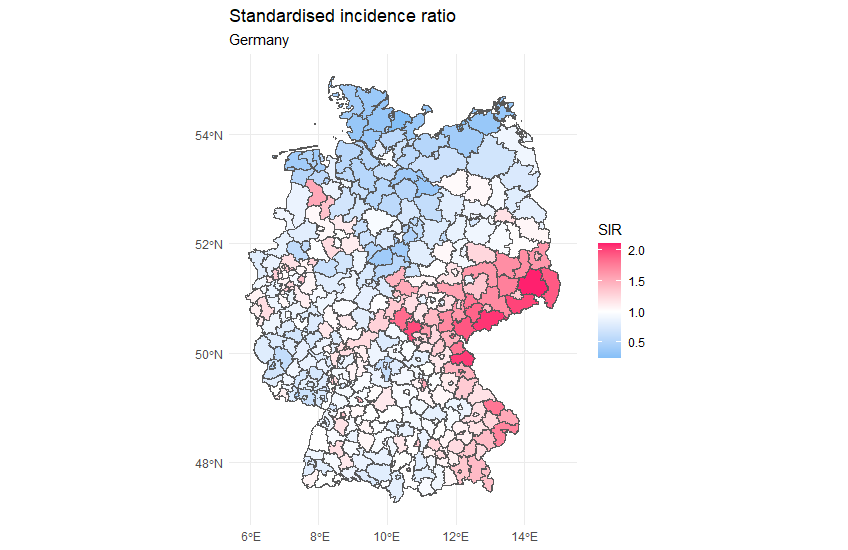
\includegraphics[width = 1.2\textwidth]{sir_germany.png}
 \caption{The SIR for Germany based on the data of the 2nd of May 2021}
 \label{sirgermany}
\end{figure}
\subsection{SIR for Norway}
Looking at the standardised incidence rate for Norway in Figure~\ref{sirnorway}, a standardised incidence rate of less than 1 can be seen for most municipalities north of Trondheim. In the southern parts of Norway there are several municipalities with a rate above 1, for example the standardised incidence rate around the capital Oslo is around 2. However, the two small municipalities, Hyllestad and Ulvik, have the highest standardised incidence rate in Norway. In Hyllestad, 95 of 1328 people have been infected with Covid-19 so far, while in Ulvik, 134 of 1080 people have been infected so far. \\
The SIR in Hyllestad is around 3.4, following an outbreak in a shipyard in autumn 2020 \cite{newspaper1}, while Ulvik has a ratio of around 5.7, following an outbreak of the UK variant of Covid-19. According to the head of the municipality, Hans Petter Thorbjørnsen, the infections are thought to have spread through children \cite{newspaper2}.
\begin{figure}[H]
 \centering
 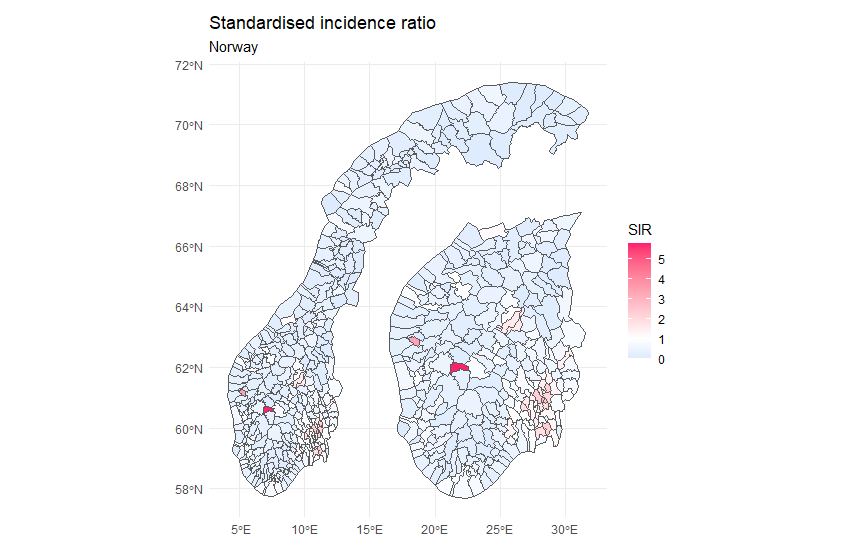
\includegraphics[width = 1.2\textwidth]{sir_norway.png}
 \caption{The SIR for Norway based on the data of the 2nd of May 2021}
 \label{sirnorway}
\end{figure}
Because the high numbers from two small municipalities complicate the interpretation of Figure~\ref{sirnorway}, Figure~\ref{sirnorwaylog} shows the SIR on a log10 scale. On this scale, a value of 0 means that the risk of infection in a given municipality is neither lower nor higher. Values below 0 mean that the risk of infection in a municipality is lower than average, while values above 1 mean that the risk of infection in a municipality is higher than average. It is now clearer that the standardized incidence ratio is below 1 in most parts of Norway, but that there is a higher risk in the region around Oslo.
\begin{figure}[H]
 \centering
 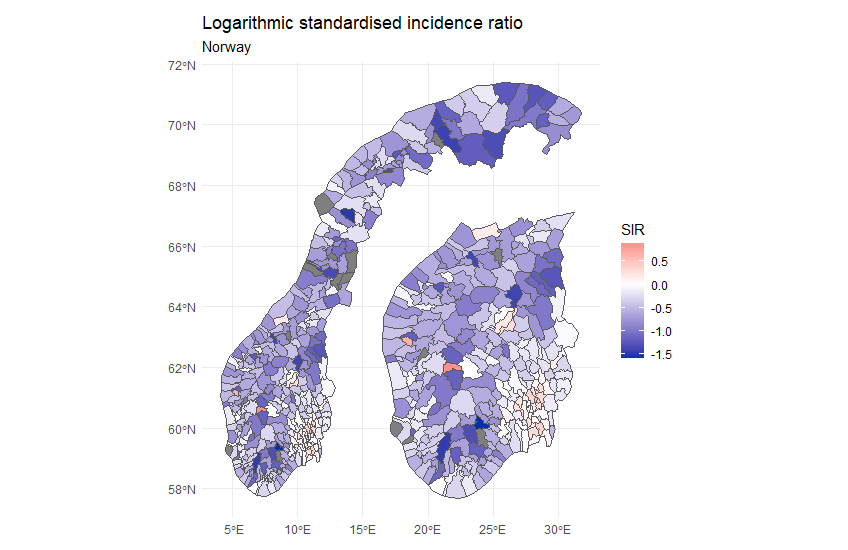
\includegraphics[width = 1.2\textwidth]{sir_norway_log.png}
 \caption{The log10 SIR for Norway based on the data of the 2nd of May 2021}
 \label{sirnorwaylog}
\end{figure}
\clearpage
\section{Data Modelling}
After looking at the standardised incidence rates for the countries of interest, the next step is to take a closer look at the current figures for the respective countries. Spatial models are used to try to extract the factors that cause some populations to be at higher risk than populations in other geographical regions. Three different types of models are used for each country:
\begin{itemize}
  \item[1.] Besags Proper Spatial Model
  \item[2.] A Leroux Model
  \item[3.] A BYM2 Model
\end{itemize}
All of these models are computed using the INLA \cite{rinla} R package. \\
To specify each type of model, the code shown in Listing~\ref{codeModels} can be used. \\
The measures introduced in Section~\ref{sec:performance}, namely the DIC, the WAIC, the CPO and the mean absolute error (MAE), are used to compare the models.\\
In addition to specifying what type of spatial model to use, if any, there is also the option of specifying a prior. \\
As can be seen in Section~\ref{sec:pc_prior}, a pc prior can be specified for the precision parameter $\tau$, which is what is done here. \\
For the parameters $\sigma_0$ and $\alpha$ in Equation~\ref{eq:pc_prior_prec} the values 1 and 0.01 are chosen. \\
The models are compared using the mean absolute error. For this, 20\% of the observations are removed from the training set and used for testing instead. The predicted number of infections for these municipalities is then compared to the actual numbers.
\\
A list of all calculated models along with their performance measures is provided in the appendix.
\subsection{Choice of Likelihood}
Before the models are computed, however, the distribution that fits the number of cases must first be found. One way to do this, the function \texttt{descdist()} from the \texttt{fitdistrplus} R package is used. The Cullen and Frey graph illustrates how "close" a sample is to a theoretical distribution based on the kurtosis and the square of the skewness, defined in Equation~\ref{eq:kurtosis} and Equation~\ref{eq:skewness}. It can be used to get a preliminary idea of which distributions fit the data, in this case the number of infections, reasonably well. \\
The plots for Germany and Norway can be seen in Figure~\ref{cf_germany} and Figure~\ref{cf_norway}. The blue dot represents the data, the star a theoretical normal distribution, the dashed line a theoretical Poisson distribution and the grey area a theoretical negative binomial distribution. In both cases, the blue dot is relatively far from the star and lies in the region of a negative binomial distribution. For the Norwegian sample shown in Figure~\ref{cf_norway}, the sample is closer to a Poisson distribution than is the case for the German sample in Figure~\ref{cf_germany}.
\begin{figure}[H]
  \centering
  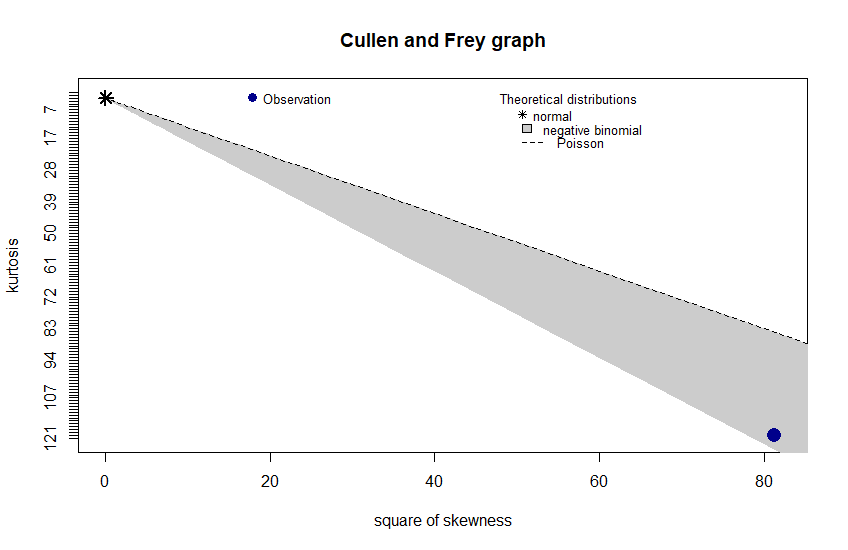
\includegraphics[width = 0.8\textwidth]{cf_germany.png}
  \caption{The Cullen and Frey graph for Germany}
  \label{cf_germany}
\end{figure}
\begin{figure}[H]
  \centering
  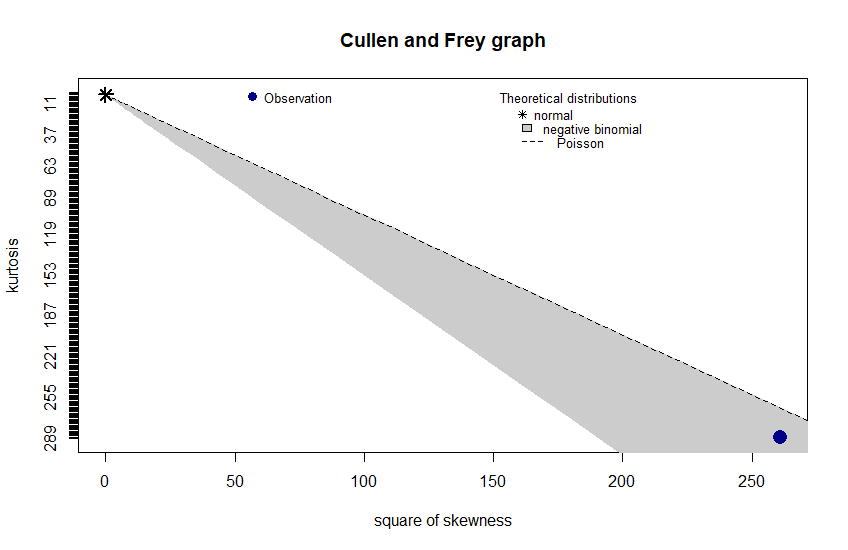
\includegraphics[width = 0.8\textwidth]{cf_norway.png}
  \caption{The Cullen and Frey graph for Norway}
  \label{cf_norway}
\end{figure}
Next, a negative binomial distribution, a normal distribution, and a Poisson distribution are fitted to the data using the maximum likelihood method. The negative binomial fits for both countries can be seen in Figure~\ref{fitNegbinomGermany} and Figure~\ref{fitNegbinomNorway}. The fits for the normal and Poisson distribution for both countries, are shown in the Appendix in Figure~\ref{fitNormalGermany}, Figure~\ref{fitPoissonGermany}, Figure~\ref{fitNormalNorway} and Figure~\ref{fitPoissonNorway}. \\
The QQ-plot for Germany and Norway looks quite similar, as there appears to be a linear relationship between the theoretical quantile and the sample quantiles, up to a certain point where the sample quantiles have a higher value than the theoretical quantiles, indicating that the distribution is right skewed. Since there are many municipalities with relatively few cases and few municipalities with a large number of cases, this is to be expected. It can also be seen that the empirical cumulative density function closely follows the theoretical cumulative density function.
\begin{figure}[H]
  \centering
  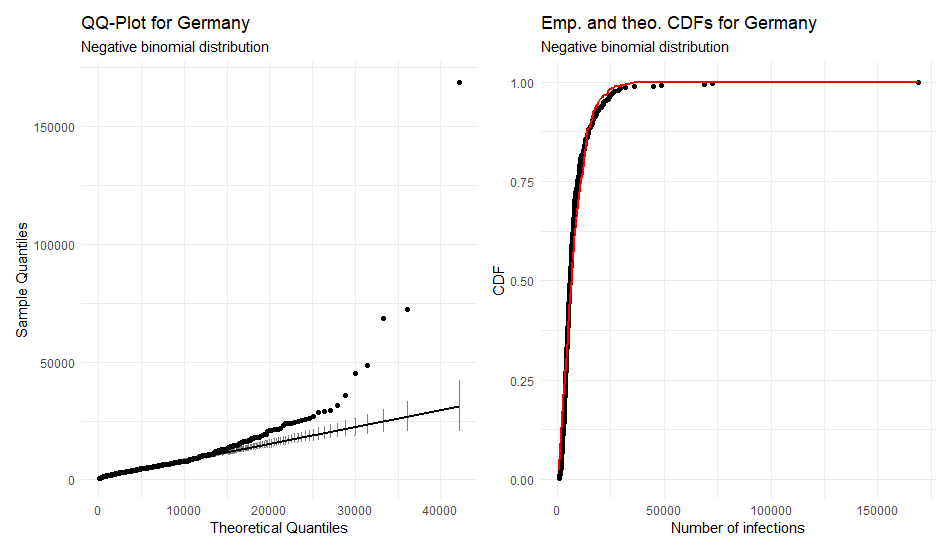
\includegraphics[width = 0.8\textwidth]{fit_nbinom_germany.png}
  \caption{A negative binomial fit to the number of cases in German municipalities}
  \label{fitNegbinomGermany}
\end{figure}
\begin{figure}[H]
  \centering
  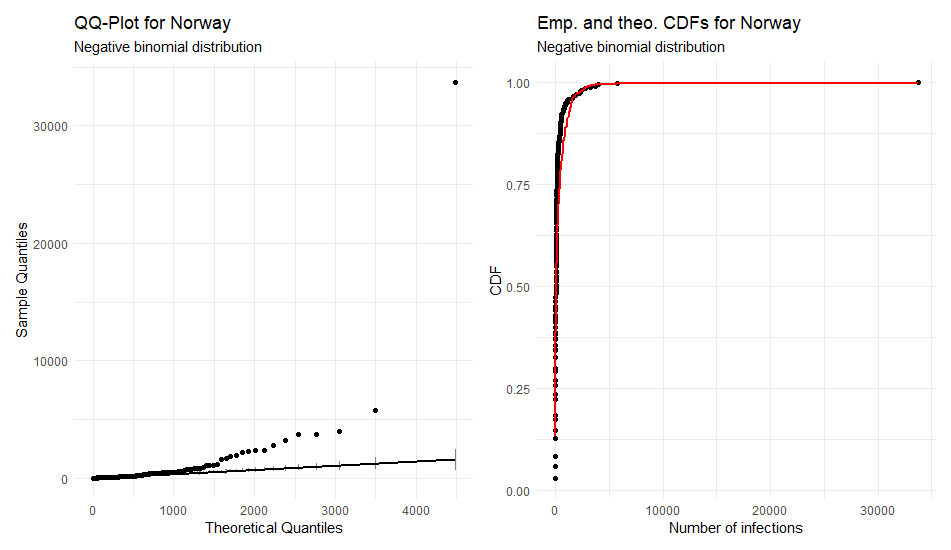
\includegraphics[width = 0.8\textwidth]{fit_nbinom_norway.png}
  \caption{A negative binomial fit to the number of cases in Norwegian municipalities}
  \label{fitNegbinomNorway}
\end{figure}
Lastly, the AIC is calculated for fitting a normal distribution to the data, a Poisson distribution to the data and a negative binomial distribution to the data. The values can be seen in Table~\ref{aic}. Afterwards, the negative binomial distribution is chosen as the distribution of the target variable in both cases. \\
\begin{table}[H] 
\caption{The AIC for different distributions for Germany and Norway \label{aic}}
\begin{tabular}{l l r}
\toprule
\textbf{Country}	& \textbf{Distribution}	& \textbf{AIC} \\
\midrule
Germany & Normal & 8619 \\
Germany & Poisson & 2699357 \\
Germany & Negative Binomial & 8010 \\
Norway & Normal & 6400 \\
Norway & Poisson & 509139 \\
Norway & Negative Binomial & 4293 \\
\bottomrule
\end{tabular}
\end{table} 
The poor fit for the Poisson distribution can be explained by looking at the range of the number of confirmed cases in a given municipality. For Germany, this number ranges from 697 to 169021 (as of May 2, 2021), while for Norway, the number ranges from 0 to 34654 (as of May 2, 2021). This results in a mean and standard deviation for Germany of 8550 and 11204, respectively. For Norway, the values for these metrics are 326 and 1930. This is problematic because, as shown in Equation~\ref{eq:poisson_exp} and Equation~\ref{eq:poisson_var}, for a Poisson distribution the expected value and the variance should be equal. \\
Looking at a histogram for the confirmed number of cases and overlaying the densities of a normal, Poisson and a negative binomial distribution helps to confirm the choice of a negative binomial distribution as the distribution that the data most closely resembles. Figure~\ref{fitDistrGermany} and Figure~\ref{fitDistrNorway} both show that a negative binomial distribution fits the data better than a normal distribution. Due to the high values for the AIC, the Poisson distribution is excluded from these graphics.
\begin{figure}[H]
  \centering
  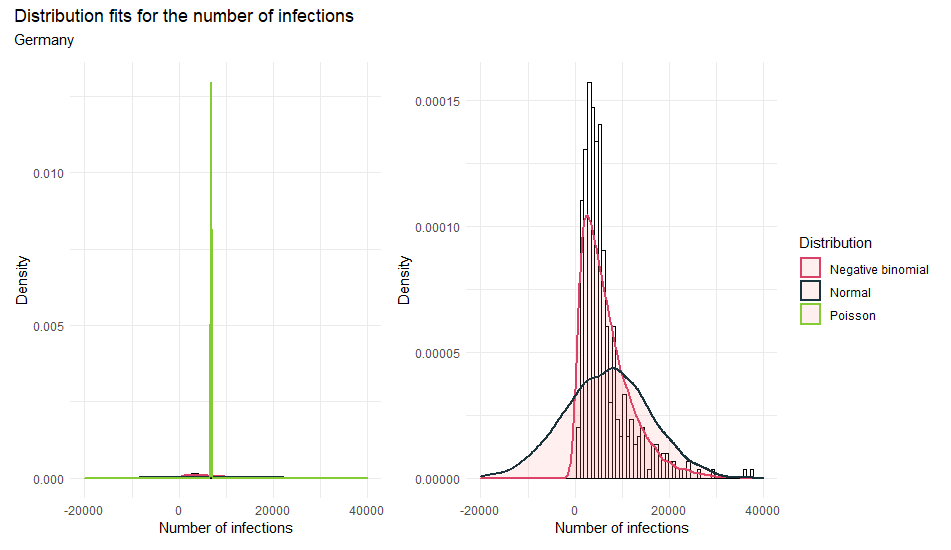
\includegraphics[width = 0.8\textwidth]{distrfit_germany.png}  
  \caption{Histogram for the number of cases in German municipalities with a normal and a negative binomial distribution overlayed.}
  \label{fitDistrGermany}
\end{figure}
\begin{figure}[H]
  \centering
  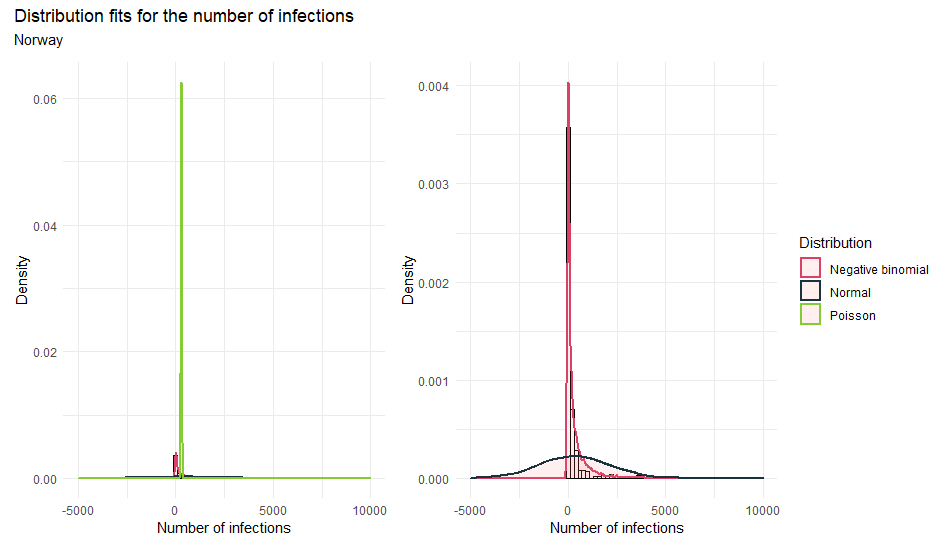
\includegraphics[width = 0.8\textwidth]{distrfit_norway.png}
  \caption{Histogram for the number of cases in Norwegian municipalities with a normal and a negative binomial distribution overlayed.}
  \label{fitDistrNorway}
\end{figure}
\clearpage
\section{Models without a Spatial Component}\label{sec:nospatial}
To establish a baseline, a look is first taken at models that do not include a spatial effect. This way, it can be observed how the means and credibility intervals of the covariates change when a spatial effect is added to a model and how the performance of the model changes with respect to the goodness-of-fit indicators introduced in Section~\ref{sec:performance}. \\
Before computing the models, using the $\hbox{VIF}$ introduced in Section~\ref{sec:vif}, predictors are removed if their $\hbox{VIF}$ is above 5. To do this, a GLM is first run on all variables, followed by the calculation of $\hbox{VIF}$. Then the variable with the highest value is removed before running the model again with all remaining variables. This process is repeated until only variables with a $\hbox{VIF}$ of less than 5 remain. \\
In sections~\ref{sec:nospatial_germany} and~\ref{sec:nospatial_norway} the results of these models are presented. Their goodness-of-fit indicators as well as the coefficients together with their credibility intervals calculated as in section~\ref{sec:mean_iv} are reported. \\
These models are based on data from 2 May 2021, when 3,428,487 people were infected with Covid-19 in Germany, while 87,537 people were infected in Norway. The five municipalities with the most infections in Germany are shown in Table~\ref{top5germany} and in Table~\ref{top5norway} for Norway.
\begin{table}[H] 
\caption{The German municipalities with the most infections as of May 2nd 2021. \label{top5germany}}
\begin{tabular}{l r r}
\toprule
\textbf{Municipality}	& \textbf{Population}	& \textbf{Number of infections} \\
\midrule
SK Berlin & 3644826 & 169021  \\   
SK Hamburg & 1841179 & 72595  \\
SK Munich & 1471508 & 68762  \\
SK Cologne & 1085664 & 48831  \\
Region Hannover & 1157624 & 45043  \\
\bottomrule
\end{tabular}
\end{table}
\begin{table}[H] 
\caption{The Norwegian municipalities with the most infections as of May 2nd 2021. \label{top5norway}}
\begin{tabular}{l r r r}
\toprule
\textbf{Municipality}	& \textbf{Population}	& \textbf{Number of infections} &\textbf{\% first vaccine shot} \\
\midrule
Oslo & 693494 & 34654 & 32.7\%\\
Bergen & 283929 & 6039 & 30.0\%\\
Drammen & 101386 & 4097 & 34.1\%\\
Bærum & 127731 & 3860 & 31.7\%\\
Lillestrøm & 85983 & 3819 & 30.2\%\\
\bottomrule
\end{tabular}
\end{table}
\subsection{Models without a Spatial Component for Germany}\label{sec:nospatial_germany}
Table~\ref{allGermany_nospatial} contains the performance measures for the baseline model for Germany, while Table~\ref{FixedAllGermany_nospatial} contains the posterior mean, the exponentiated posterior mean and the credibility intervals of the coefficients. It can be seen that the intercept as well as six of the coefficients are significant.
\begin{table}[H] 
\caption{The performance measures for the model without a spatial component. \label{allGermany_nospatial}}
\begin{tabular}{r r r r}
\toprule
\textbf{DIC}	& \textbf{WAIC} & \textbf{CPO} & \textbf{MAE}\\
\midrule
5595 & 5598 & -2816 & 182174 \\
\bottomrule
\end{tabular}
\end{table}
\begin{table}[H]
\caption{The fixed effects for the model. Values are rounded. A $^*$ denotes a significant effect. \label{FixedAllGermany_nospatial}}
\begin{tabular}{l r r r r c}
\toprule
\textbf{Variable}	& \textbf{mean$_{\hbox{p}}$}	& \textbf{exp(mean$_{\hbox{p}}$)} & \textbf{exp(q0025$_{\hbox{p}}$)} & \textbf{exp(q0975$_{\hbox{p}}$)} & \textbf{sig.}\\
\midrule
(Intercept) & -0.1494 & 0.9602 & 0.9363 & 0.9846 & $^*$\\
AfD & 0.1788 & 1.198 & 1.062 & 1.346 & $^*$\\
Population & \multirow{2}{*}{0.1567} & \multirow{2}{*}{1.170} & \multirow{2}{*}{1.117} & \multirow{2}{*}{1.226} & \multirow{2}{*}{$^*$}\\
density \\
Logarithmic & \multirow{2}{*}{0.08418} & \multirow{2}{*}{1.088} & \multirow{2}{*}{1.041} & \multirow{2}{*}{1.136} & \multirow{2}{*}{$^*$}\\
trade tax \\
Platform & 0.03655 & 1.038 & 0.9880 & 1.089 \\
Die Union & 0.03169 & 1.035 & 0.8967 & 1.188\\
Higher & \multirow{2}{*}{0.01797} & \multirow{2}{*}{1.018} & \multirow{2}{*}{0.9806} & \multirow{2}{*}{1.058} \\
Education\\
Sex & 0.01615 & 1.016 & 0.9843 & 1.049 & \\
Urban density & 0.008459 & 1.009 & 0.9725 & 1.047 \\
FDP & 0.007239 & 1.007 & 0.9722 & 1.044 \\
Place of & \multirow{2}{*}{-0.003902} & \multirow{2}{*}{0.9963} & \multirow{2}{*}{0.9549} & \multirow{2}{*}{1.039} \\
worship\\
Nursing & \multirow{2}{*}{-0.01245} & \multirow{2}{*}{0.9878} & \multirow{2}{*}{0.9586} & \multirow{2}{*}{1.018} \\
home\\
Clinic & -0.01257 & 0.9878 & 0.9396 & 1.039 \\
Aerodrome & -0.01432 & 0.9859 & 0.9542 & 1.019 \\
Office & -0.02943 & 0.9712 & 0.9304 & 1.015 \\
Marketplace & -0.04434 & 0.9570 & 0.9048 & 1.011 \\
SPD & -0.08652 & 0.9178 & 0.8502 & 0.9890 & $^*$\\
The left & -0.1173 & 0.8900 & 0.8231 & 0.9610 & $^*$\\
Greens & -0.1494 & 0.8630 & 0.7575 & 0.9789 & $^*$\\
\bottomrule
\end{tabular}
\end{table}
\subsection{Models without a Spatial Component for Norway}\label{sec:nospatial_norway}
Table~\ref{allNorway_nospatial} contains the performance measures for the baseline model for Germany, while Table~\ref{fixedAllNorway_nospatial} contains the posterior mean, the exponentiated posterior mean and the credibility intervals of the coefficients. It can be seen that the intercept as well as five of the coefficients are significant.
\begin{table}[H] 
\caption{The performance measures for the model without a spatial component. \label{allNorway_nospatial}}
\begin{tabular}{r r r r}
\toprule\textbf{DIC}	& \textbf{WAIC} & \textbf{CPO} & \textbf{MAE}\\
\midrule
2830 & 2835 & -1689 & 7986 \\
\bottomrule
\end{tabular}
\end{table} 
\begin{table}[H]
\caption{The fixed effects for the model. Values are rounded. A $^*$ denotes a significant effect. \label{fixedAllNorway_nospatial}}
\begin{tabular}{l r r r r c}
\toprule
\textbf{Variable}	& \textbf{mean$_{\hbox{p}}$}	& \textbf{exp(mean$_{\hbox{p}}$)} & \textbf{exp(q0025$_{\hbox{p}}$)} & \textbf{exp(q0975$_{\hbox{p}}$)} & \textbf{sig.}\\
\midrule
(Intercept) & -0.8305 & 0.4363 & 0.3994 & 0.4764 & $^*$ \\
Unemployed & \multirow{2}{*}{0.2291} & \multirow{2}{*}{1.262} & \multirow{2}{*}{1.077} & \multirow{2}{*}{1.475} & \multirow{2}{*}{$^*$} \\
immigrants\\
Total & \multirow{2}{*}{0.2080}& \multirow{2}{*}{1.234}& \multirow{2}{*}{1.079}& \multirow{2}{*}{1.407}& \multirow{2}{*}{$^*$}\\
immigrants \\
Urban density & 0.1881 & 1.211 & 1.049 & 1.413 & $^*$ \\
Total & \multirow{2}{*}{0.1119} & \multirow{2}{*}{1.125} & \multirow{2}{*}{0.9094} & \multirow{2}{*}{1.382} \\
unemployment \\
Vaccinations & 0.07299 & 1.078 & 0.9600 & 1.206\\
Marketplace & 0.04402 & 1.046 & 0.9526 & 1.159 \\
Platform & 0.03983 & 1.043 & 0.9070 & 1.204 \\
Higher & \multirow{2}{*}{0.02369}& \multirow{2}{*}{1.025}& \multirow{2}{*}{0.9429}& \multirow{2}{*}{1.129}\\ 
education \\
Nursing & \multirow{2}{*}{0.01011} & \multirow{2}{*}{1.011} & \multirow{2}{*}{0.9302} & \multirow{2}{*}{1.115} \\
home\\
Place of\_ & \multirow{2}{*}{-0.02375}& \multirow{2}{*}{0.9793}& \multirow{2}{*}{0.8456}& \multirow{2}{*}{1.136} \\
worship \\
Median age & -0.04400 & 0.9588 & 0.8480 & 1.079 \\
Aerodrome & -0.1276 & 0.8812 & 0.8022 & 0.9682 & $^*$ \\
Office & -0.1536 & 0.8604 & 0.7359 & 1.008 \\
Sex & -0.1644 & 0.8499 & 0.7559 & 0.9524 & $^*$ \\
\bottomrule
\end{tabular}
\end{table}
\clearpage
\section{Spatial Models}\label{ch:spatial}
Looking at the SIR value for Germany in Figure~\ref{sirgermany} and the SIR value for Norway in Figure~\ref{sirnorway} and Figure~\ref{sirnorwaylog}, it clearly looks like there is a correlation between the SIR and the spatial units. For Germany, the SIR is higher in eastern Germany than in the rest of the country and in Norway the risk seems to be mainly concentrated around the Oslo region. \\
To check whether there is spatial autocorrelation, Moran's I, introduced in Section~\ref{sec:moran}, can be calculated and the Moran test can then be used to tell whether there is spatial autocorrelation. Under the null hypothesis of no spatial autocorrelation, a p-value greater than 0.05 would be expected. The results of the test are presented in Table~\ref{moranTest}. Looking at the p-value for both countries, it can be seen that the number of infections in a municipality and the spatial units are correlated.
\begin{table}[H] 
\caption{Results of the Moran test for Germany and Norway. \label{moranTest}}
\begin{tabular}{l r r r r}
\toprule
\textbf{Country} & \textbf{Moran's I}	& \textbf{$\mathbb{E}\left[I\right]$}	& \textbf{p-Value} \\
\midrule
Germany & 0.1096 & -0.002500 & < 0.01 \\
Norway & 0.1083 & -0.002817 & < 0.01 \\
\bottomrule
\end{tabular}
\end{table}
Therefore, after the models without spatial effect have been calculated and established as baseline models, a spatial term is added to the models calculated in Section~\ref{sec:nospatial} , in order to model this spatial correlation.
\subsection{Spatial Models for Germany}
Looking at the performance of the spatial models and the model with the spatial component shown in Table~\ref{allGermany}, it can be seen that the spatial models perform better in terms of the DIC, WAIC and MAE, while they perform equally well or better in terms of the CPO. \\
The best performance of all models, in terms of MAE, was observed for the BYM2 model, which slightly outperformed the Besag model.
\begin{table}[H] 
\caption{The performance measures for the best performing model of each type. \label{allGermany}}
\begin{tabular}{l r r r r}
\toprule
\textbf{Model}	& \textbf{DIC}	& \textbf{WAIC} & \textbf{CPO} & \textbf{MAE}\\
\midrule
No spatial & 5595 & 5598 & -2816 & 182174 \\
Besag& 4832 & 4875 & -2802 & 179229\\
BYM2 & 4732 & 4705 & -2751 & 179181\\
Leroux & 4818 & 4882 & -2919 & 184348 \\
\bottomrule
\end{tabular}
\end{table}
Figure~\ref{intervalGermany} shows the differences between the coefficients in the model without the spatial component and the BYM2 model. Excluding the intercept, only three effects are significant in the BYM2 model compared to six in the model without the spatial component. Moreover, the coefficients of the BYM2 model are closer to 1. 
\begin{figure}[H]
  \centering
  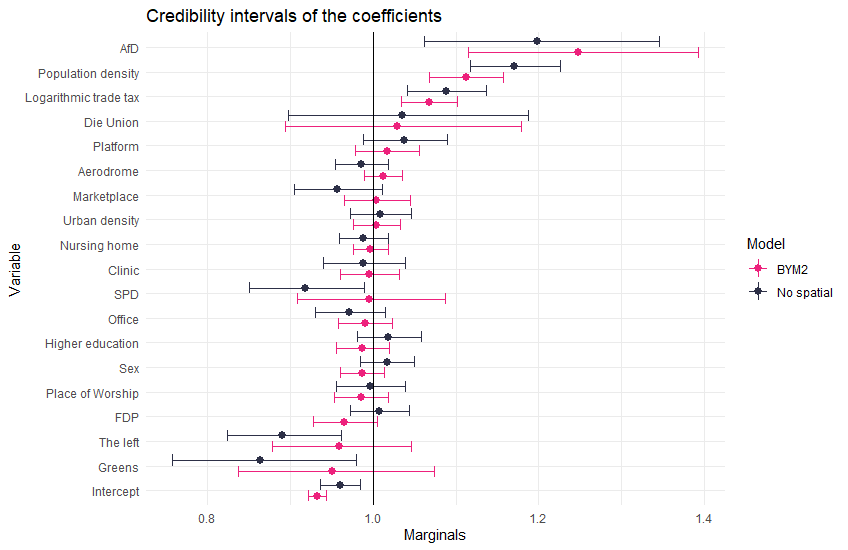
\includegraphics[width = \textwidth]{intervals_germany.png}
  \caption{The posterior mean and credibility intervals of the coefficients}
  \label{intervalGermany}
\end{figure}
The values of the coefficients and credibility intervals are shown in Table~\ref{FixedAllGermany_spatial}.
\begin{table}[H]
\caption{The fixed effects for the model. Values are rounded. A $^*$ denotes a significant effect. \label{FixedAllGermany_spatial}}
\begin{tabular}{l r r r r c}
\toprule
\textbf{Variable}	& \textbf{mean$_{\hbox{p}}$}	& \textbf{exp(mean$_{\hbox{p}}$)} & \textbf{exp(q0025$_{\hbox{p}}$)} & \textbf{exp(q0975$_{\hbox{p}}$)} & \textbf{sig.}\\
\midrule
(Intercept) & -0.07023 & 0.9322 & 0.9214 & 0.9433 & $^*$\\
AfD & 0.2200 & 1.248 & 1.114 & 1.393 & $^*$\\
Population & \multirow{2}{*}{0.1058} & \multirow{2}{*}{1.112} & \multirow{2}{*}{1.068} & \multirow{2}{*}{1.157} & \multirow{2}{*}{$^*$}\\
density \\
Logarithmic & \multirow{2}{*}{0.06494} & \multirow{2}{*}{1.067} & \multirow{2}{*}{1.034} & \multirow{2}{*}{1.101} & \multirow{2}{*}{$^*$}\\
Trade tax \\
Die Union & 0.02625 & 1.029 & 0.8937 & 1.179\\
Platform & 0.01619 & 1.017 & 0.9781 & 1.056 \\
Aerodrome & 0.01192 & 1.012 & 0.9894 & 1.035 \\
Marketplace & 0.003678 & 1.004 & 0.9646 & 1.044 \\
Urban density & 0.003663 & 1.004 & 0.9756 & 1.032 \\
Nursing& \multirow{2}{*}{-0.003431} & \multirow{2}{*}{0.9966} & \multirow{2}{*}{0.9754} & \multirow{2}{*}{1.018} \\
Home\\
Clinic & -0.004643 & 0.9955 & 0.9600 & 1.032 \\
SPD & -0.006260 & 0.9948 & 0.9080 & 1.085\\
Office & -0.01021 & 0.9900 & 0.9578 & 1.023 \\
Higher & \multirow{2}{*}{-0.01335} & \multirow{2}{*}{0.9869} & \multirow{2}{*}{0.9551} & \multirow{2}{*}{1.019} \\
Education\\
Sex & -0.01359 & 0.9866 & 0.9601 & 1.014 & \\
Place of & \multirow{2}{*}{-0.01497} & \multirow{2}{*}{0.9853} & \multirow{2}{*}{0.9532} & \multirow{2}{*}{1.018} \\
Worship\\
FDP & -0.03553 & 0.9653 & 0.9271& 1.005 \\
The left & -0.04276 & 0.9591 & 0.8776 & 1.046\\
Greens & -0.05333 & 0.9500 & 0.8372 & 1.073 \\
\bottomrule
\end{tabular}
\end{table}
For the hyperparameters, a value of 18.61 is reported for the precision and a value of 0.9032 for $\phi$. Hence, 90.32\% of the marginal variance is explained by the structured effect. Therefore, this model is far from reducing to pure overdispersion and comes close to a Besag model, which is also reflected in the similar values of the goodness-of-fit indicators in Table~\ref{allGermany}.
\subsection{Spatial Models for Norway}
Comparing the performance of the models, the spatial models again showed better performance in terms of DIC and WAIC and this time also significantly better performance in terms of CPO. However, the model without the spatial component showed better predictive performance, as indicated by the lowest value for the MAE in Table~\ref{allNorway}. This could indicate that neighbourhood effects are not as strong in Norway as in Germany.
\begin{table}[H] 
\caption{The performance measures for the best performing model of each type. \label{allNorway}}
\begin{tabular}{l r r r r}
\toprule
\textbf{Model}	& \textbf{DIC}	& \textbf{WAIC} & \textbf{CPO} & \textbf{MAE} \\
\midrule
No spatial & 2830 & 2835 & -1689 & 7986 \\
Besag & 2824 & 2830 & -2099 & 8186 \\
BYM2 & 2780 & 2787 & -4387 & 8344\\
Leroux & 2359 & 2340 & -4820 & 8691\\
\bottomrule
\end{tabular}
\end{table}
Looking at the differences between the coefficients and credibility intervals in Figure~\ref{intervalNorway}, the picture is similar to Figure~\ref{intervalGermany}. This time, however, all significant effects of the model without the spatial component are still significant. This again shows that the spatial effect is weaker in Norway than in Germany, as no new variables turn out to be significant and no variables lose their significance when the spatial term is added.
\begin{figure}[H]
  \centering
  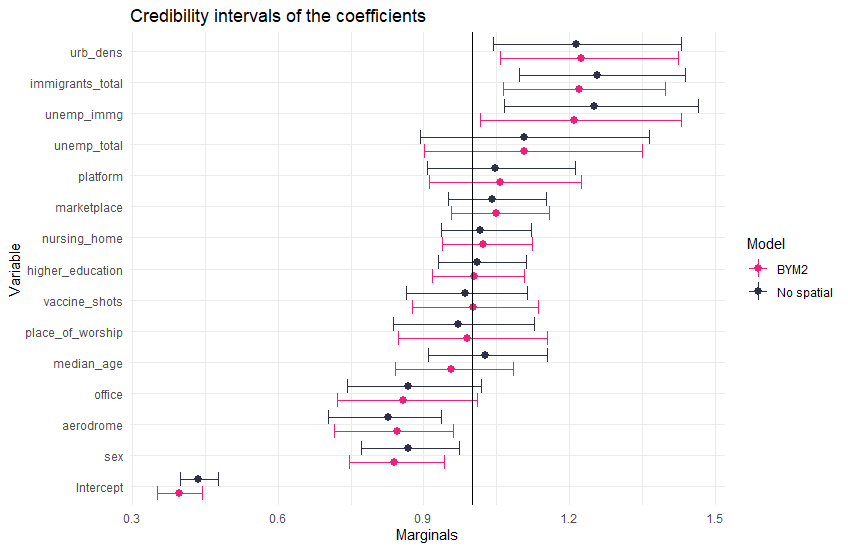
\includegraphics[width = \textwidth]{intervals_norway.png}
  \caption{The posterior mean and credibility intervals of the coefficients}
  \label{intervalNorway}
\end{figure}
The values of the coefficients and credibility intervals are shown in Table~\ref{fixedAllNorway_spatial}.
\begin{table}[H]
\caption{The fixed effects for the model. Values are rounded. A $^*$ denotes a significant effect. \label{fixedAllNorway_spatial}}
\begin{tabular}{l r r r r c}
\toprule
\textbf{Variable}	& \textbf{mean$_{\hbox{p}}$}	& \textbf{exp(mean$_{\hbox{p}}$)} & \textbf{exp(q0025$_{\hbox{p}}$)} & \textbf{exp(q0975$_{\hbox{p}}$)} & \textbf{sig.}\\
\midrule
(Intercept) & -0.9387 & 0.3919 & 0.3448 & 0.4397 & $^*$ \\
Urban density & 0.2001 & 1.225 & 1.064 & 1.415 & $^*$ \\
Unemployed & \multirow{2}{*}{0.1851} & \multirow{2}{*}{1.208} & \multirow{2}{*}{1.017} & \multirow{2}{*}{1.425} & \multirow{2}{*}{$^*$} \\
immigrants\\
Total & \multirow{2}{*}{0.1825}& \multirow{2}{*}{1.203}& \multirow{2}{*}{1.052}& \multirow{2}{*}{1.371}& \multirow{2}{*}{$^*$}\\
immigrants \\
Total & \multirow{2}{*}{0.1145}& \multirow{2}{*}{1.127}& \multirow{2}{*}{0.9209}& \multirow{2}{*}{1.367}\\
unemployment \\
Vaccinations & 0.07554 & 1.080 & 0.9592 & 1.211\\
Marketplace & 0.04588 & 1.048 & 0.9546 & 1.156 \\
Platform & 0.04438 & 1.048 & 0.9053 & 1.211\\
Higher & \multirow{2}{*}{0.02068}& \multirow{2}{*}{1.022}& \multirow{2}{*}{0.9312}& \multirow{2}{*}{1.128}\\ 
education \\
Nursing & \multirow{2}{*}{0.01626} & \multirow{2}{*}{1.017} & \multirow{2}{*}{0.9326} & \multirow{2}{*}{1.117} \\
home\\
Place of & \multirow{2}{*}{-0.002547}& \multirow{2}{*}{1.001}& \multirow{2}{*}{0.8572}& \multirow{2}{*}{1.166} \\
worship \\
Median age& -0.1054 & 0.9018 & 0.7939 & 1.020 \\
Aerodrome & -0.3110 & 0.8783 & 0.7968 & 0.9664 & $^*$ \\
Office & -0.1641 & 0.8518 & 0.7187 & 1.003 \\
Sex & -0.2022 & 0.8184 & 0.7285 & 0.9158 & $^*$ \\
\bottomrule
\end{tabular}
\end{table}
For the hyperparameters, a value of 5.398 is reported for the precision and a value of 0.1295 for $\phi$. Hence, 12.95\% of the marginal variance is explained by the structured effect. Therefore, this model is close to pure overdispersion.
\clearpage
\section{Choice of Hyperpriors}
As can be seen in Equation~\ref{pcprec}, there is flexibility when it comes to choosing the values for the standard deviation $\sigma_0$ as well as the probability $\alpha$. Therefore, an upper bound for the standard deviation can be chosen as well as the weight placed on this "tail event", describing how informative the resulting prior is. \\
Some of the issues that come with the choice of these hyperpriors were already discussed in Section~\ref{sec:issues}. \\
In the following, an assessment is made of how the performance of a Besag model, a BYM2 model and a Leroux model changes when playing around with the value for the standard deviation $\sigma_0$. To create these plots, models were calculated with $\sigma_0$ values of $\pmb{\sigma_0}=\left(0.1,0.11,0.12,...,5\right)$.\\
In Figure~\ref{comparison_norway_1} it can be seen that when choosing a higher value for $\sigma_0$, the DIC and WAIC is lower in the case of the Besag model and the BYM2 model. For the Leroux model, on the other hand, the WAIC gets lower until about 2 before it rises until around $\sigma_0 = 2.5$ and then flattens out. It is a positive sign that this is not the case with the BYM2 model, as it was designed to avoid exactly this kind of thing. \\
For the CPO and MAE in Figure~\ref{comparison_norway_2}, it can be seen that for all model types, a higher value for $\sigma_0$ leads to a higher MAE.
\begin{figure}[H]
  \centering
  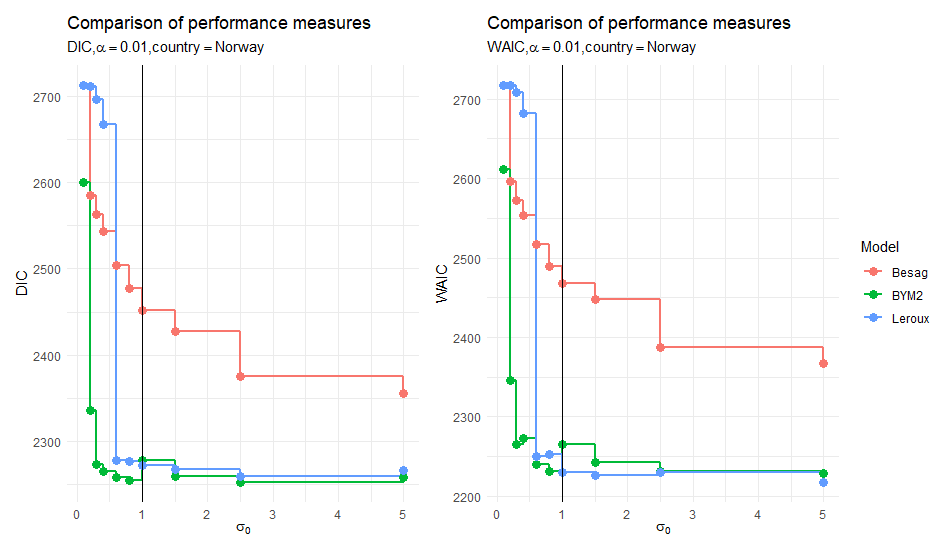
\includegraphics[width = \textwidth]{comparison_1_norway.png}
  \caption{Values of the DIC and the WAIC when changing the value for $\sigma_0$. The black line highlights the values for $\sigma_0$ = 1.}
  \label{comparison_norway_1}
\end{figure}
\begin{figure}[H]
  \centering
  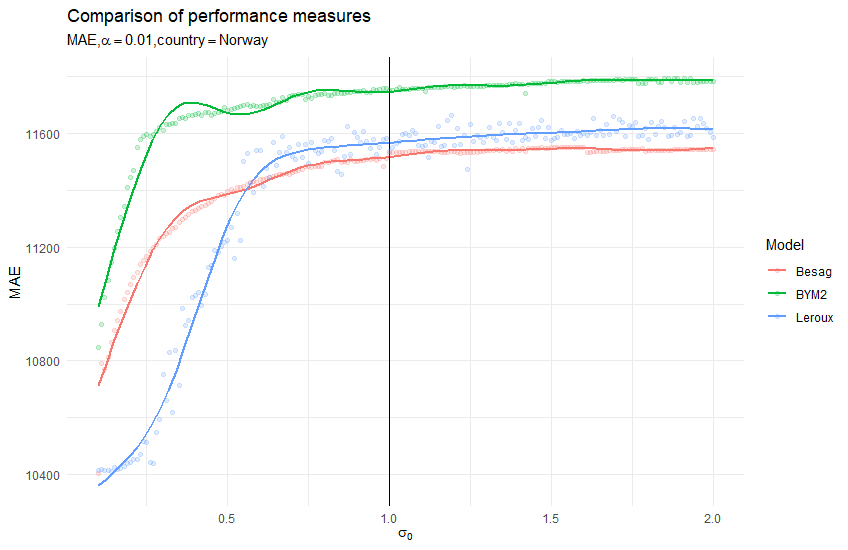
\includegraphics[width = \textwidth]{mae_norway.png}
  \caption{Value of the MAE when changing the value for $\sigma_0$. The black line highlights the values for $\sigma_0$ = 1.}
  \label{comparison_norway_2}
\end{figure}
By allowing the precision to be greater, the variance is forced to be smaller. Hence, choosing a lower value for the precision leads to lower values for the WAIC. While this indicates a better fit to the training data, Figure~\ref{comparison_norway_2} also shows that the MAE increases when a higher value for $\sigma_0$ is chosen, as the models overfit on the training data and therefore make worse predictions. \\
The corresponding figures for Germany are shown in Figure~\ref{comparison_germany_1} and Figure~\ref{comparison_germany_2} in the Appendix. \\
Figure~\ref{comparison_norway_5} shows how the credibility intervals of the coefficients of a BYM2 model change when the value for $\sigma_0$ is increased. The values of the coefficients tend to remain relatively similar most of the time, especially when the value of the coefficient is close to 1. However, a few times, for example for the variables immigrants\_total, platform and unemp\_immg, the values differ. Furthermore, the coefficients for $\sigma_0 = 1$ and $\sigma_0 = 2$ are more closer to 1 than the ones for $\sigma_0=0.1$.
\begin{figure}[H]
  \centering
  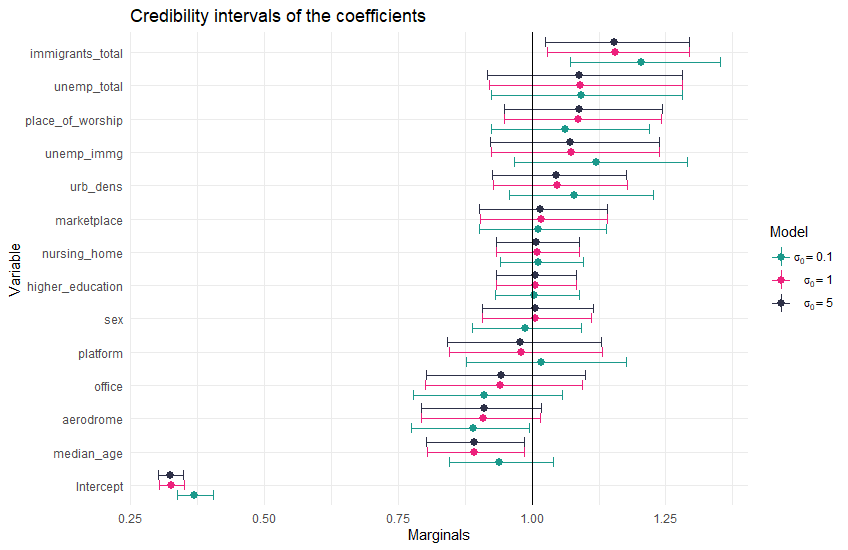
\includegraphics[width = \textwidth]{intervals_prior_norway.png}
  \caption{Comparison of the credibility intervals of a BYM2 model for different values of $\sigma_0$.}
  \label{comparison_norway_5}
\end{figure}
Having credibility intervals and posterior means that are very similar to each other, regardless of the value chosen for $\sigma_0$, is a great sign as it means that the calculated model is robust. That is, it means that the fixed covariates are important in their own right because they provide different information than the spatial field, even if the spatial field is allowed to be very smooth or coarse. This is exactly the case for Germany, which can be seen in Figure~\ref{comparison_germany_5}.
\begin{figure}[H]
    \centering
    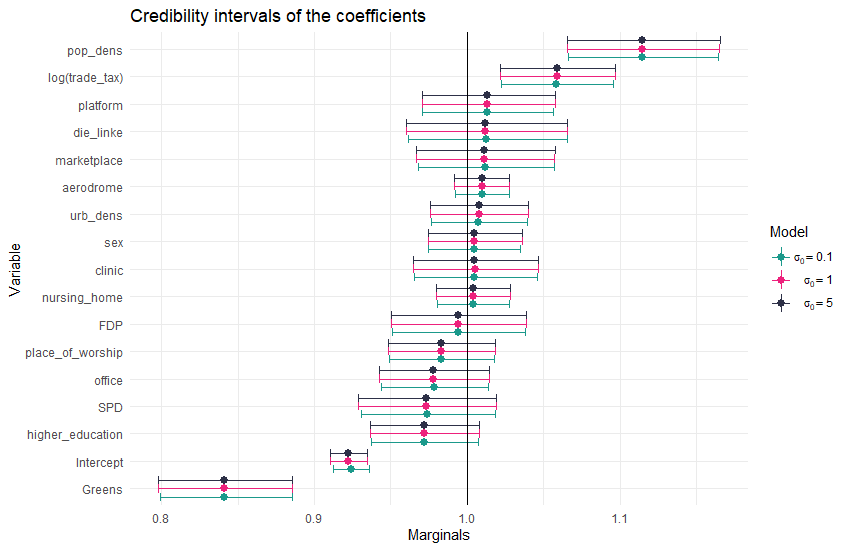
\includegraphics[width = \textwidth]{intervals_prior_germany.png}
    \caption{Comparison of the credibility intervals of a BYM2 model for different values of $\sigma_0$}
    \label{comparison_germany_5}
\end{figure}
Figure~\ref{comparison_norway_6} and Figure~\ref{comparison_norway_7} underline the problem of the models not being comparable with each other. Figure~\ref{comparison_norway_6} already shows huge differences in the spatial field of the Besag model and the Leroux model, with the spatial field of the Besag model looking smoother than the spatial field of the Leroux model. This is a sign that the Leroux model is quickly overfitting to the data.
In the left part of Figure~\ref{comparison_norway_7} the values of Equation~\ref{eq:bym2_1} are plotted, while in the right part the values of $u_{*}$ are plotted. \\
For the spatial field of the unstructured random effect, the values of the posterior mean are similar to the values of the Besag model. For the structured component, however, the absolute values are somewhat higher. Nevertheless, in both cases the values are far from the values for the Leroux model.
\begin{figure}[H]
  \centering
  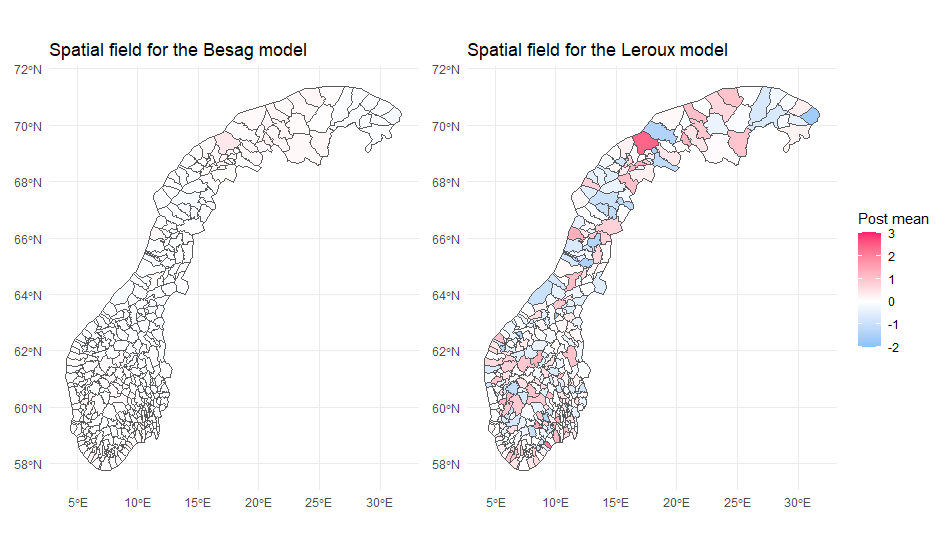
\includegraphics[width = \textwidth]{spatial_field_norway_1.png}
  \caption{Spatial field for a Besag model and a Leroux model.}
  \label{comparison_norway_6}
\end{figure}
\begin{figure}[H]
  \centering
  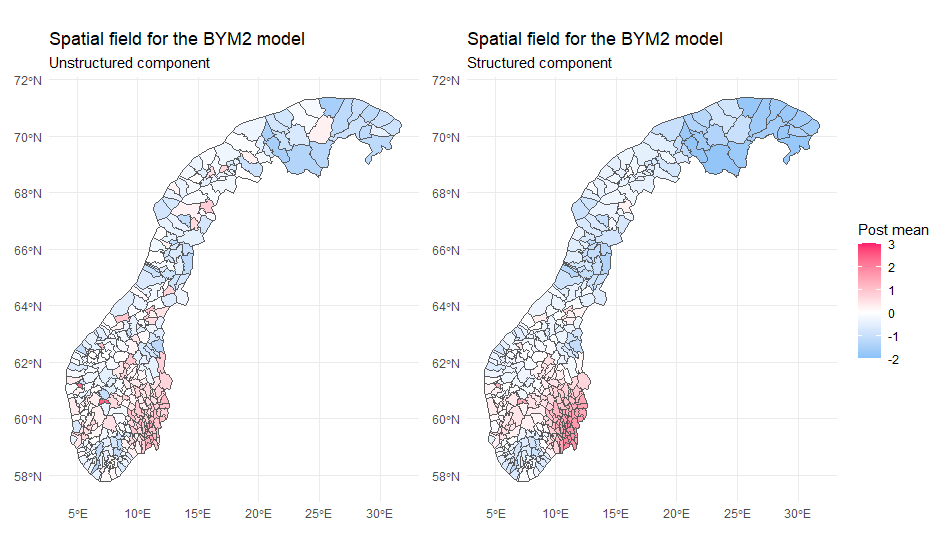
\includegraphics[width = \textwidth]{spatial_field_norway_2.png}
  \caption{Spatial fields for a BYM2 model.}
  \label{comparison_norway_7}
\end{figure}
The corresponding figures for Germany are shown in Figure~\ref{comparison_germany_6} and Figure~\ref{comparison_germany_7} in the Appendix. \\
Finally, looking at the spatial field of the structured component when changing the value for $\sigma_0$, as seen in Figure~\ref{comparison_norway_8}, it can be seen that for a small value like $\sigma_0 = 0.1$, the values of the posterior mean are mostly around 0, while for a higher value these values get slightly higher. The reason for this is simply that higher values for $\sigma_0$ make the spatial field fit the data more closely, making it less smooth.
\begin{figure}[H]
  \centering
  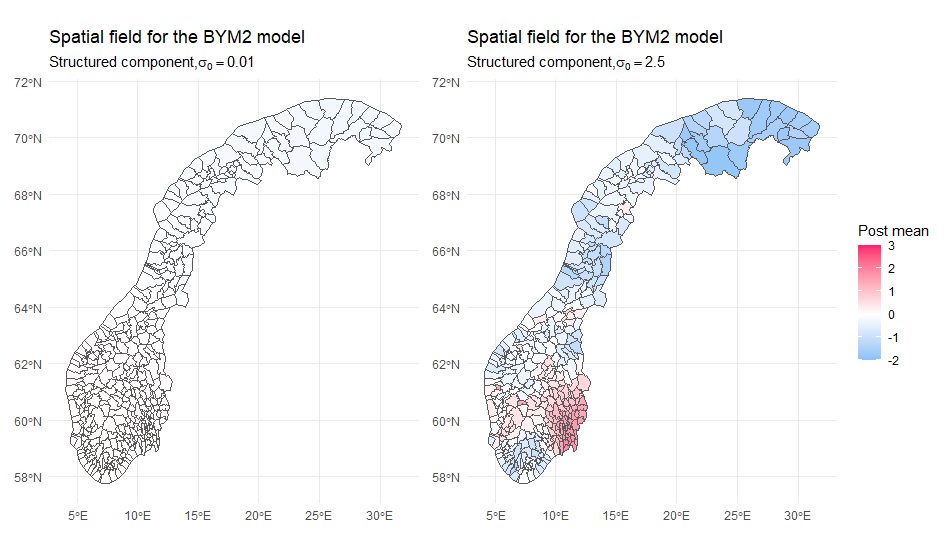
\includegraphics[width = \textwidth]{spatial_field_norway_3.png}
  \caption{Spatial fields for the structured component of a BYM2 model when changing the value for $\sigma_0$.}
  \label{comparison_norway_8}
\end{figure}
Looking at Figure~\ref{comparison_germany_8}, there are hardly any differences in the spatial fields for $\sigma_0=0,1$ and $\sigma_0=2$, which again shows how robust the model is for Germany.
\begin{figure}[H]
    \centering
    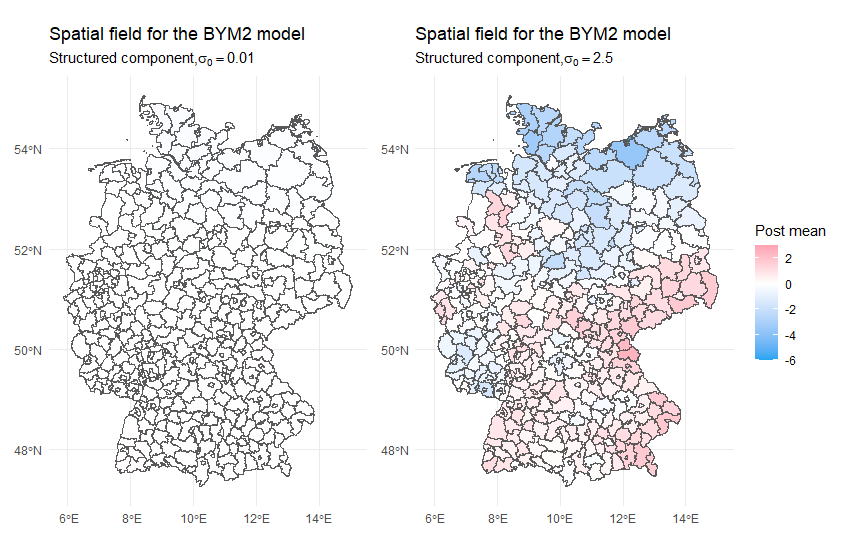
\includegraphics[width = \textwidth]{spatial_field_germany_3.png}
    \caption{Spatial fields for the structured component of a BYM2 model when changing the value for $\sigma_0$.}
    \label{comparison_germany_8}
\end{figure}

\clearpage
\section{Spatio-Temporal Models}
\subsection{Spatio-Temporal Models for Germany}
\begin{table}[H] 
\caption{The German municipalities with the most infections as of May 2nd 2021. \label{top5Germany_temporal}}
\begin{tabular}{l r r r}
\toprule
\textbf{Municipality}	& \textbf{Population}	& \textbf{Number of infections} \\
\midrule
SK Berlin & 3644826 & 165450 \\
SK Hamburg & 1841179 & 70903 \\
SK Munich & 1471508 & 66951 \\
SK Cologne & 1085664 & 47007 \\
Region Hannover & 1157624 & 43665 \\
\bottomrule
\end{tabular}
\end{table}
\begin{table}[H] 
\caption{The performance measures for the best performing model of each type. \label{allGermany_temporal}}
\begin{tabular}{l r r r r}
\toprule
\textbf{Model}	& \textbf{DIC}	& \textbf{WAIC} & \textbf{CPO} & \textbf{MAE} \\
\midrule
No spatial & 5606 & 5609 & -2831 & 178621 \\
Spatial BYM2 & 4743 & 4742 & -2806 & 175619\\
Besag & 371291 & 371346 & -185605 & 204410 \\
BYM2 & 371291 & 371348 & -185605 & 204369\\
Leroux & 371283 & 371353 & -185609 & 204434\\
\bottomrule
\end{tabular}
\end{table}
\begin{figure}[H]
  \centering
  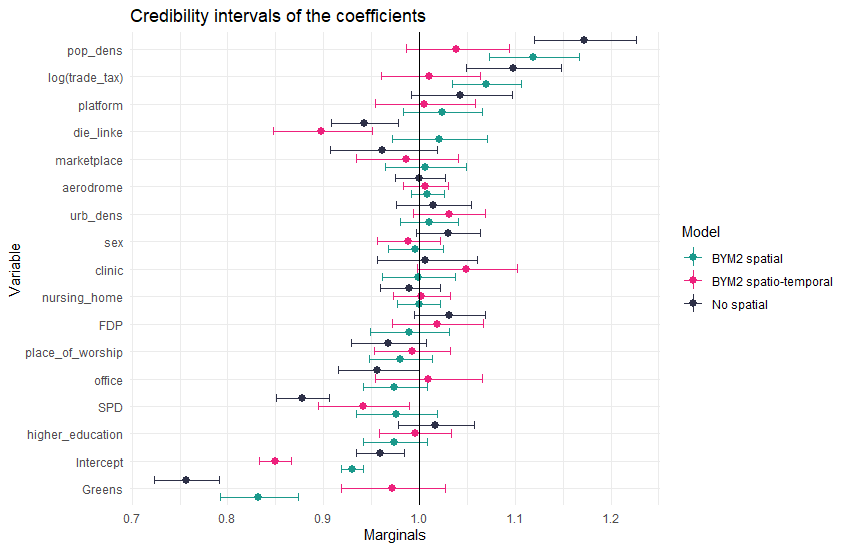
\includegraphics[width = \textwidth]{intervals_germany_temporal.png}
  \caption{The posterior mean and credibility intervals of the coefficients}
  \label{intervalGermany_temporal}
\end{figure}
\begin{table}[H]
\caption{The fixed effects for the model. Values are rounded. A $^*$ denotes a significant effect. \label{fixedAllGermany_temporal}}
\begin{tabular}{l r r r r c}
\toprule
\textbf{Variable}	& \textbf{mean$_{\hbox{p}}$}	& \textbf{exp(mean$_{\hbox{p}}$)} & \textbf{exp(q0025$_{\hbox{p}}$)} & \textbf{exp(q0975$_{\hbox{p}}$)} & \textbf{sig.}\\
\midrule
(Intercept) & -0.1633 & 0.8494 & 0.8326 & 0.8662 & $^*$\\
clinic & 0.04774 & 1.049 & 0.9978 & 1.103 \\
pop\_dens & 0.03800 & 1.039 & 0.9862 & 1.094 \\
urb\_dens & 0.03051 & 1.031 & 0.9940 & 1.069 \\
FDP & 0.01803 & 1.018 & 0.9720 & 1.067 \\
log & \multirow{2}{*}{0.01034} & \multirow{2}{*}{1.011} & \multirow{2}{*}{0.9604} & \multirow{2}{*}{1.063} & \multirow{2}{*}{}\\
trade\_tax \\
office & 0.008501 & 1.009 & 0.9538 & 1.066 \\
aerodrome & 0.006449 & 1.007 & 0.9831 & 1.030 \\
platform & 0.004554 & 1.005 & 0.9536 & 1.058 \\
nursing\_ & \multirow{2}{*}{0.002101} & \multirow{2}{*}{1.002} & \multirow{2}{*}{0.9726} & \multirow{2}{*}{1.032} \\
home\\
higher\_ & \multirow{2}{*}{-0.004663} & \multirow{2}{*}{0.9955} & \multirow{2}{*}{0.9585} & \multirow{2}{*}{1.034} \\
education\\
place\_of\_ & \multirow{2}{*}{-0.007753} & \multirow{2}{*}{0.9925} & \multirow{2}{*}{0.9533} & \multirow{2}{*}{1.033} \\
worship\\
sex & -0.01148 & 0.9887 & 0.0.9565 & 1.022 \\
marketplace & -0.01395 & 0.9865 & 0.9340 & 1.041 \\
Greens & -0.02903 & 0.9718 & 0.9188 & 1.027\\
SPD & -0.06109 & 0.9410 & 0.8944 & 0.9892 & $^*$ \\
die\_linke & -0.1081 & 0.8980 & 0.8471 & 0.9508& $^*$ \\
\bottomrule
\end{tabular}
\end{table}
For the hyperparameters, a value of 12.59 is reported for the precision of the area and 26950740 for the precision of the date, A value of 0.6989 is reported for $\phi$. Hence, 69.89\% of the marginal variance is explained by the structured effect. Therefore, this model is closer to a Besag model than it is to overdispersion.
\begin{figure}[H]
  \centering
  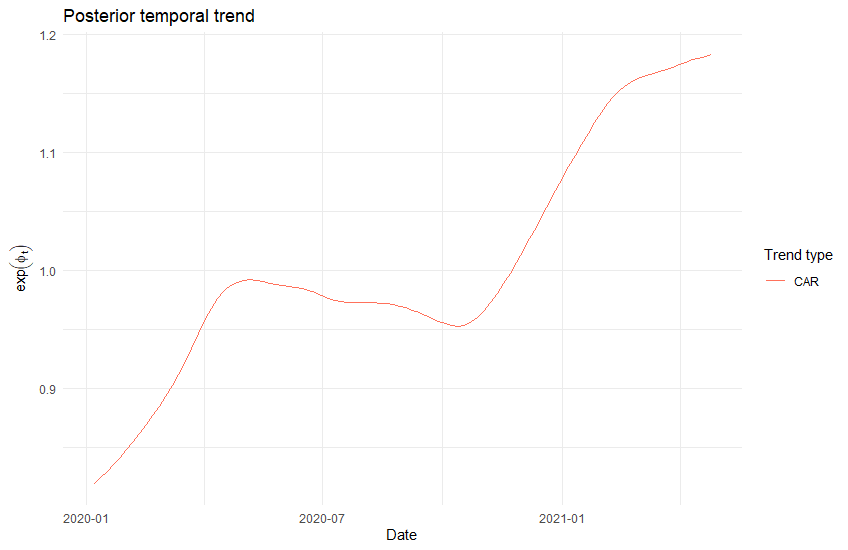
\includegraphics[width = \textwidth]{temporal_trend_germany.png}
  \caption{The temporal trend of the BYM2 model.}
  \label{temporal_trend_germany}
\end{figure}
\begin{figure}[H]
  \centering
  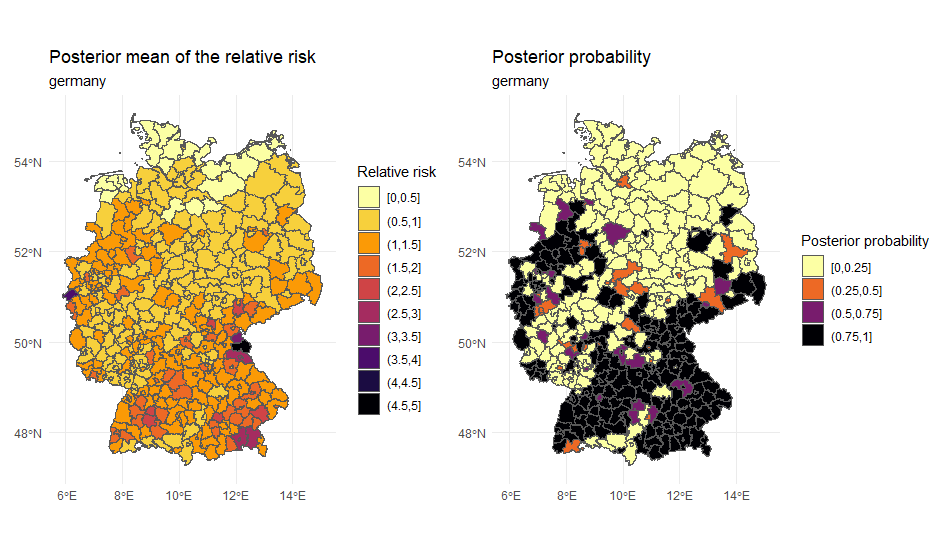
\includegraphics[width = \textwidth]{posterior_germany_temporal.png}
  \caption{Posterior mean of the area-specific risk and the posterior probability.}
  \label{posterior_germany_temporal}
\end{figure}
\subsection{Spatio-Temporal Models for Norway}
\begin{table}[H] 
\caption{The Norwegian municipalities with the most infections as of May 2nd 2021. \label{top5norway_temporal}}
\begin{tabular}{l r r r}
\toprule
\textbf{Municipality}	& \textbf{Population}	& \textbf{Number of infections} &\textbf{\% first vaccine shot} \\
\midrule
Oslo & 693494 & 33296 & 32.7\%\\
Bergen & 283929 & 5701 & 30.0\%\\
Drammen & 101386 & 3956 & 34.1\%\\
Bærum & 127731 & 3726 & 31.7\%\\
Lillestrøm & 85983 & 3725 & 30.2\%\\
\bottomrule
\end{tabular}
\end{table}
\begin{table}[H] 
\caption{The performance measures for the best performing model of each type. \label{allNorway_temporal}}
\begin{tabular}{l r r r r}
\toprule
\textbf{Model}	& \textbf{DIC}	& \textbf{WAIC} & \textbf{CPO} & \textbf{MAE} \\
\midrule
No spatial & 2813 & 2817 & -1662 & 7686 \\
Spatial BYM2 & 2777 & 2783 & -4065 & 7943\\
Besag & 130574 & 130545 & -65273 & 11376 \\
BYM2 & 130572 & 130543 & -65272 & 11376\\
Leroux & 130574 & 130545 & -65273 & 11377\\
\bottomrule
\end{tabular}
\end{table}
\begin{figure}[H]
  \centering
  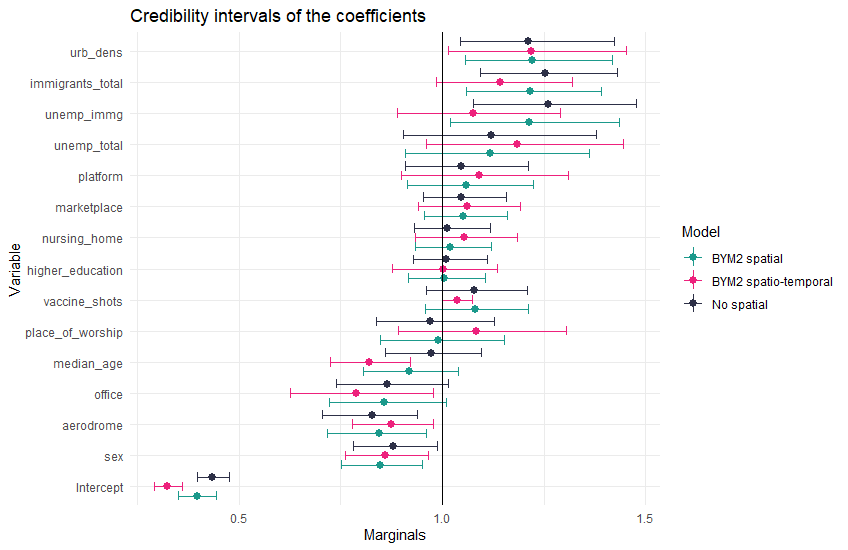
\includegraphics[width = \textwidth]{intervals_norway_temporal.png}
  \caption{The posterior mean and credibility intervals of the coefficients}
  \label{intervalNorway_temporal}
\end{figure}
\begin{table}[H]
\caption{The fixed effects for the model. Values are rounded. A $^*$ denotes a significant effect. \label{fixedAllNorway_temporal}}
\begin{tabular}{l r r r r c}
\toprule
\textbf{Variable}	& \textbf{mean$_{\hbox{p}}$}	& \textbf{exp(mean$_{\hbox{p}}$)} & \textbf{exp(q0025$_{\hbox{p}}$)} & \textbf{exp(q0975$_{\hbox{p}}$)} & \textbf{sig.}\\
\midrule
(Intercept) & -1.127 & 0.3244 & 0.2917 & 0.3594 & $^*$ \\
urb\_dens & 0.1946 & 1.220 & 1.015 & 1.453 & $^*$ \\
unemp\_tot & 0.1637 & 1.184 & 0.9596 & 1.445 \\
immigrants\_ & \multirow{2}{*}{0.1310}& \multirow{2}{*}{1.143}& \multirow{2}{*}{0.9856}& \multirow{2}{*}{1.318}& \multirow{2}{*}{}\\
total \\
platform & 0.08178 & 1.090 & 0.8996 & 1.309 \\
place\_of\_ & \multirow{2}{*}{0.07557}& \multirow{2}{*}{1.084}& \multirow{2}{*}{0.8907}& \multirow{2}{*}{1.306} \\
worship \\
unemp\_ & \multirow{2}{*}{0.06943} & \multirow{2}{*}{1.077} & \multirow{2}{*}{0.8897} & \multirow{2}{*}{1.291} & \multirow{2}{*}{} \\
immg\\
marketplace & 0.05738 & 1.061 & 0.9409 & 1.192 \\
nursing\_ & \multirow{2}{*}{0.05047} & \multirow{2}{*}{1.054} & \multirow{2}{*}{0.9338} & \multirow{2}{*}{1.185} \\
home\\
vaccine\_shots & 0.03609 & 1.037 & 1.001 & 1.074 & $^*$\\
higher\_ & \multirow{2}{*}{-0.001071}& \multirow{2}{*}{1.001}& \multirow{2}{*}{0.8780}& \multirow{2}{*}{1.136}\\ 
education \\
aerodrome & -0.1367 & 0.8738 & 0.7777 & 0.9779 & $^*$ \\
sex & -0.1538 & 0.8591 & 0.7606 & 0.9662 & $^*$ \\
median\_age & -0.2013 & 0.8192 & 0.7244 & 0.9223 &$^*$ \\
office & -0.2455 & 0.7874 & 0.6254 & 0.9777 & $^*$ \\
\bottomrule
\end{tabular}
\end{table}
For the hyperparameters, a value of 0.9783 is reported for the precision of the area and 5471899 for the precision of the date, A value of 0.02769 is reported for $\phi$. Hence, 2.77\% of the marginal variance is explained by the structured effect. Therefore, this model is very close to pure overdispersion.
\begin{figure}[H]
  \centering
  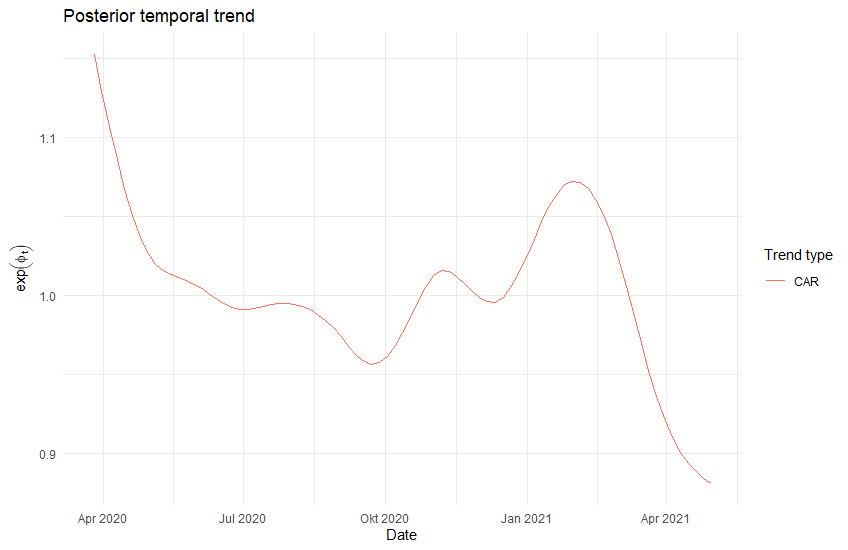
\includegraphics[width = \textwidth]{temporal_trend_norway.png}
  \caption{The temporal trend of the BYM2 model.}
  \label{temporal_trend_norway}
\end{figure}
\begin{figure}[H]
  \centering
  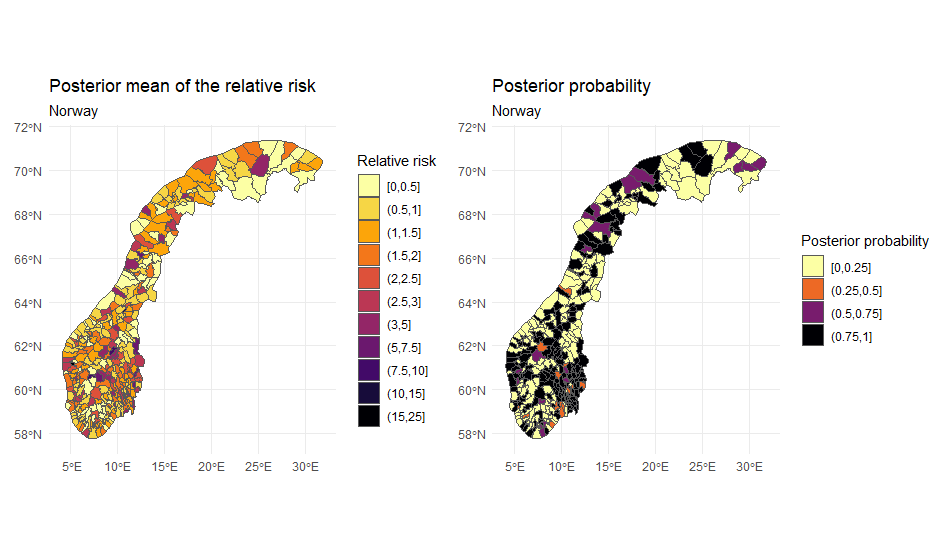
\includegraphics[width = \textwidth]{posterior_norway_temporal.png}
  \caption{Posterior mean of the area-specific risk and the posterior probability.}
  \label{posterior_norway_temporal}
\end{figure}
\begin{figure}[H]
  \centering
  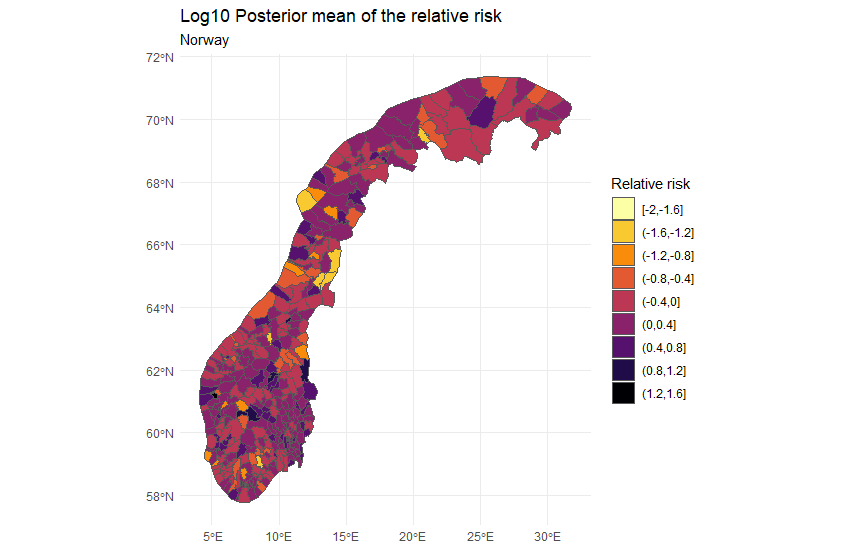
\includegraphics[width = \textwidth]{posterior_norway_temporal_log.png}
  \caption{Log posterior mean of the area-specific risk.}
  \label{posterior_norway_temporal_log}
\end{figure}
\clearpage
\section{Predictive Models}
\subsection{Predictive Models for Germany}
\subsection{Predictive Models for Norway}